% siminos/atlas/symm.tex  pdflatex atlas
% $Author$ $Date$


\section{What is a symmetry?}
\label{s:symm}

    \ifdraft\color{blue}
Argue: symmetry, non-shape changing  drifts are cheap, as they are not
shape changing and burn no energy
    \color{black}\fi

A flow $\dot{\ssp}= \vel(\ssp)$ is said to be $\Group$-\emph{equivariant}
if the form of evolution equations \refeq{symbolicNS} is left invariant
by the set of transformations $\LieEl$ that form the group of symmetries
of the dynamics $\Group$,
\beq
\vel(\ssp)=\LieEl^{-1} \, \vel(\LieEl \, \ssp)
\,,\qquad \mbox{for all } \LieEl \in {\Group}
\,.
\ee{eq:FiniteRot}
While the flow equations are invariant under $\Group$, the state of flow
typically is not. Only the laminar Hagen-Poiseuille \eqv\ is invariant
under all of $\Group$, whereas a generic turbulent state has only the
trivial symmetry group $\{e\}$.

\subsection{Ring of Fire}

%%%%%%%%%%%%%%%%%%%%%%%%%%%%%%%%%%%%%%%%%%%%%%%%%%%%%%%%%%%%%%%%%%%%%
\begin{figure}
(a) 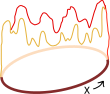
\includegraphics[width=0.15\textwidth]{A27RoFire}
(b) 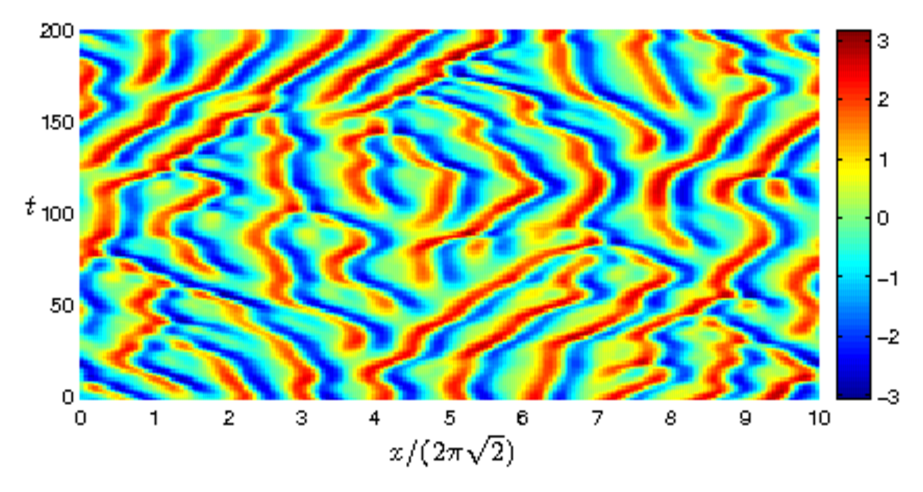
\includegraphics[width=0.25\textwidth]{ks_largeL_cbar_200}
  \caption{
The Ring of Fire, visualized as
    (a)
a Bunsen burner flame flutter, with $u=u(x,t)$ the velocity of the
flame front at position $x$ and time $t$;
    (b)
a spatiotemporal plot (from \wwwcb{}). The symmetry of the system is
$\On{2}$; a rotation of a solution is also a solution.
  }
\label{fig:A27RoFir}
\end{figure}
%%%%%%%%%%%%%%%%%%%%%%%%%%%%%%%%%%%%%%%%%%%%%%%%%%%%%%%%%%%%%%%%%%%%%

Bunsen burner, invented by G\"ottingen chemistry prodigy Robert Bunsen in
1855, entered popular culture in  in 1963 as Johnny Cash
\etal\rf{CaCaKi63} ``\HREF{http://www.youtube.com/watch?v=mIBTg7q9oNc}
{Ring of Fire}'' (\reffig{fig:A27RoFir}), and its flame front
instabilities were modeled in 1976 by Kuramoto\rf{ku} and
Sivashinsky\rf{siv} by one of the simplest nonlinear PDEs that exhibit
spatiotemporally chaotic behavior. The time evolution of the  flame front
velocity $u=u(x,t)$ on a periodic domain $u(x,t) = u(x+L,t)$ is given by
\beq
  u_t = F(u) = -u\,u_x-u_{xx}-u_{xxxx}
    \,.
\ee{ks}
Spatial periodicity $u(x,t)=u(x+L,t)$
makes it convenient to work in the Fourier space,
\beq
  u(x,t)=\sum_{k=-\infty}^{+\infty} a_k (t)\, e^{ i k x /\tildeL }
\,,
\ee{eq:ksexp}
with the $1$-dimensional PDE \refeq{ks}
replaced by an infinite set of
ODEs for the complex Fourier coefficients $a_k(t)$:
\beq
\dot{a}_k= \pVeloc_k(a)
     = ( q_k^2 - q_k^4 )\, a_k
    - i \frac{q_k}{2} \sum_{m=-\infty}^{+\infty} a_m a_{k-m}
\,,
\ee{expan}
where $q_k = 2\pi k/L$.

\subsection{Pipes and planes}

 %% A27*-pipeSymms.* - read dasbuch/book/FigSrc/inkscape/00ReadMe.txt
 \begin{figure}
 \begin{center}
  \setlength{\unitlength}{0.20\textwidth}
  %% \unitlength = units used in the Picture Environment
(a)
  \begin{picture}(1,0.52454249)%
    \put(0,0){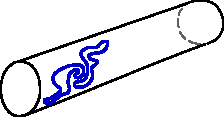
\includegraphics[width=\unitlength]{A27a-pipeSymms}}%
    \put(0.61583231,0.13683004){\color[rgb]{0,0,0}\makebox(0,0)[lb]{\smash{$z$}}}%
    \put(0.00611823,0.27217453){\color[rgb]{0,0,0}\makebox(0,0)[lb]{\smash{$\theta$}}}%
  \end{picture}%
(b)
  \begin{picture}(1,0.52454249)%
    \put(0,0){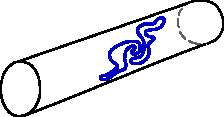
\includegraphics[width=\unitlength]{A27b-pipeSymms}}%
    \put(0.61583231,0.13683004){\color[rgb]{0,0,0}\makebox(0,0)[lb]{\smash{$z$}}}%
    \put(0.00611823,0.27217453){\color[rgb]{0,0,0}\makebox(0,0)[lb]{\smash{$\theta$}}}%
  \end{picture}%
\\
(c)
  \begin{picture}(1,0.52454249)%
    \put(0,0){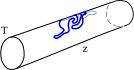
\includegraphics[width=\unitlength]{A27c-pipeSymms}}%
    \put(0.61583231,0.13683004){\color[rgb]{0,0,0}\makebox(0,0)[lb]{\smash{$z$}}}%
    \put(0.00611823,0.27217453){\color[rgb]{0,0,0}\makebox(0,0)[lb]{\smash{$\theta$}}}%
  \end{picture}%
(d)
  \begin{picture}(1,0.52454249)%
    \put(0,0){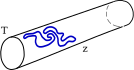
\includegraphics[width=\unitlength]{A27d-pipeSymms}}%
    \put(0.61583231,0.13683004){\color[rgb]{0,0,0}\makebox(0,0)[lb]{\smash{$z$}}}%
    \put(0.00611823,0.27217453){\color[rgb]{0,0,0}\makebox(0,0)[lb]{\smash{$\theta$}}}%
  \end{picture}%
 \end{center}
 \caption{\label{fig:A27-pipeSymms}
$\On{2}_\theta \times \SOn{2}_z$ symmetry of pipe flow: A \rpo\ $p$ is a
state of the fluid
 (a)
that reappears
 (b)
period $\period{}$ later, translated by downstream shift $\shift$
(in contrast to a \reqv, a constant shape that travels
downstream with constant {\phaseVel} $\velRel$); such solutions are
stream-wise $\SOn{2}_z$ equivariant; or
 (c)
period $\period{}$ later, translated by downstream shift $\shift$
and rotated azimuthaly by $\gSpace_p$; $\SOn{2}_{\theta} \times \SOn{2}_z$
equivariant; or
 (d)
period $\period{}$ later, reflected and rotated azimuthaly by
$\gSpace$; $\On{2}_{\theta}$ equivariant
(from \wwwcb{}).
 }%
 \end{figure}
													\toCB
The symmetry group $\Gpipe$ of stream-wise periodic pipe flow contains
two commuting \SOn{2} rotations (\reffig{fig:A27-pipeSymms}). Each
\SOn{2} group orbit is topologically a
circle (\reffig{fig:2840GOt135th0}), and together they sweep out a
contorted $T^2$ torus
(\reffig{fig:2830GO6}).

\subsection{\CLe}


\section{Group action}

\subsection{Finite shifts}

The \emph{group orbit} $\pS_\ssp $ of a \statesp\ point $\ssp \in \pS$ is
traced out by the set of all group actions
\beq
\pS_\ssp = \{\LieEl\,\ssp \mid \LieEl \in {\Group}\}
% \,,\qquad \pS_\ssp \subset \pS
\,.
\ee{sspOrbit}
Any state in the  group orbit set $\pS_{\ssp}$
is physically equivalent to any other. The action of a symmetry group
thus foliates the \statesp\ into a union of group orbits,
\reffig{fig:BeThTraj}\,(a).

\subsection{Eqs of motion}
\subsection{Infinitesimal, Jacobian derivative}
\subsection{Moving frame}

 %% A27*-pipeSymms.* - read dasbuch/book/FigSrc/inkscape/00ReadMe.txt
 \begin{figure}
 \begin{center}
  \setlength{\unitlength}{0.20\textwidth}
  %% \unitlength = units used in the Picture Environment
(a)
  \begin{picture}(1,0.95721498)%
    \put(0,0){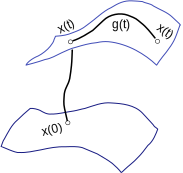
\includegraphics[width=\unitlength]{A27movFrame}}%
    \put(0.23395329,0.20526921){\color[rgb]{0,0,0}\rotatebox{13.70564637}{\makebox(0,0)[lb]{\smash{$\ssp(0)$}}}}%
    \put(0.33020326,0.77255567){\color[rgb]{0,0,0}\rotatebox{25.42186498}{\makebox(0,0)[lb]{\smash{$\ssp(\zeit)$}}}}%
    \put(0.86118813,0.79527003){\color[rgb]{0,0,0}\rotatebox{-35.54161781}{\makebox(0,0)[lb]{\smash{$\sspRed(\zeit)$}}}}%
    \put(0.61793265,0.80204565){\color[rgb]{0,0,0}\makebox(0,0)[lb]{\smash{$\LieEl(\zeit)$}}}%
  \end{picture}%
(b)
  \begin{picture}(1,0.95956879)%
    \put(0,0){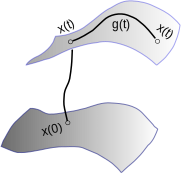
\includegraphics[width=\unitlength]{A27movFrame1}}%
    \put(0.23452859,0.20577397){\color[rgb]{0,0,0}\rotatebox{13.70564637}{\makebox(0,0)[lb]{\smash{$\ssp(0)$}}}}%
    \put(0.33101524,0.7744554){\color[rgb]{0,0,0}\rotatebox{25.42186498}{\makebox(0,0)[lb]{\smash{$\ssp(\zeit)$}}}}%
    \put(0.8633058,0.79722561){\color[rgb]{0,0,0}\rotatebox{-35.54161781}{\makebox(0,0)[lb]{\smash{$\sspRed(\zeit)$}}}}%
    \put(0.61945216,0.80401789){\color[rgb]{0,0,0}\makebox(0,0)[lb]{\smash{$\LieEl(\zeit)$}}}%
  \end{picture}%
 \end{center}
 \caption{\label{fig:A27movFrame}
$\On{2}_\theta \times \SOn{2}_z$ symmetry of pipe flow: A \rpo\ $p$ is a
state of the fluid
 (a)
that reappears
 (b)
period $\period{p}$ later, translated by downstream shift $\shift_p$
(in contrast to a \reqv, a constant shape that travels
downstream with constant {\phaseVel} $\velRel$); such solutions are
stream-wise $\SOn{2}_z$ equivariant; or
 (c)
period $\period{p}$ later, translated by downstream shift $\shift_p$
and rotated azimuthaly by $\gSpace_p$; $\SOn{2}_{\theta} \times \SOn{2}_z$
equivariant; or
 (d)
period $\period{p}$ later, reflected and rotated azimuthaly by
$\gSpace_p$; $\On{2}_{\theta}$ equivariant
(from \wwwcb{}).
 }%
 \end{figure}
													\toCB
    \PC{
Use \reffig{fig:A27movFrame} in ChaosBook.org and siminos/atlas/atlas.tex.
(to Predrag: remember to copy them to dabook/book/Fig and FigSrc/).
How it was drawn is described in
dasbuch/book/FigSrc/inkscape/00ReadMe.txt
    }
For a time-dependent group parameter
$\gSpace$, the phase speed $\dot{\gSpace}$ along the group tangent
evaluated at the \statesp\ point $\ssp$ (the `Cartan derivative') is
given by
\beq
\LieEl^{-1}\dot{\LieEl} \,\ssp % =e^{-\gSpace \cdot \Lg} \,
     =\mathrm{e}^{-\gSpace \Lg} \,
\left(\frac{\mathrm{d} ~~}{\mathrm{d} \, \zeit} \, % e^{\gSpace \cdot \Lg}\ssp
                             \mathrm{e}^{\gSpace \Lg}\right)\ssp
    =\dot{\gSpace} \, \groupTan(\ssp)
%    =\dot{\gSpace}\cdot \groupTan(\ssp)
\,.
\ee{CartanDer}

\subsection{Symmetry-induced coordinate frames}
\label{s:symmIndCoo}

At least locally, presence of a continuous symmetry suggests two
natural mutually orthogonal basis vectors, the group action tangent and
curvature vectors.

Consider the one-parameter rotation group \SOn{2} acting on a smooth
periodic function $u(\gSpace + 2\pi) = u(\gSpace)$ defined on domain
$\gSpace \in [0,2\pi)$, expanded in the Fourier basis
\refeq{eq:ksexp}.
    \PC{replace this by the original, 2\dmn\  real \SOn{2}  representation}
Parametrize the forward
translation by the continuous parameter $\phi$,
\(
    \LieEl(\phi)\,u(\gSpace) = u(\gSpace-\phi)
\,,
\)
or, in the Fourier basis,
\(
   \LieEl(\phi) \,\ssp = \mathrm{diag}\{ \mathrm{e}^{-\mathrm{i}m\phi} \} \,\ssp
\,.
\)
The tangent to the group orbit at the point $\ssp$ is then given by
the first derivative with respect to the group parameter,
The tangent to the group orbit at the point $\ssp$ is then given by
the first derivative with respect to the group parameter,
and the direction of curvature by the second derivative,
\bea
   {\bf t}(\ssp) &=&
   \lim_{\gSpace\to 0}
   \left(\LieEl(\gSpace)\,\ssp - \ssp\right)/\gSpace
   = \mathrm{diag}\{ -\mathrm{i}m \} \, \ssp = \Lg \ssp,
\label{eq:tang}\\
   \kappa(\ssp)\, {\bf n}(\ssp) &=& \Lg^2 \ssp  = - \mathrm{diag}\{m^2\} \, \ssp
   \,,
\label{eq:curv}
\eea
where $\normVec$ is a unit vector normal to the tangent and
$1/\kappa$ is the radius of curvature. The pair of unit vectors
    \PC{2011-10-28
    ``As $\Norm{\LieEl(\gSpace)\slicep}$ is a constant, for the group tangent
    vector $\Lg_\gSpace \slicep$ evaluated at $\slicep$ \refeq{eq:tang}
    %GroupTangField} is normal to $\slicep$, and the term
    $\braket{\slicep}{\Lg_\theta\,\slicep}$ vanishes ($\Lg_{\theta}$ is
    antisymmetric).''
The state vector $\ssp$ is not normal to \normVec(\ssp), as $\braket{\ssp
\Lg^2}{\ssp} = - \Norm{\groupTan(\ssp)}^2 \neq 0$, but can one use it to
produce from $\ssp$ the 3. local eigenbasis unit vector? Have not thought
that through. If we do that here, need to rewrite text leading to
\refeq{PCsectQ0}.
    }
\beq
\{{\be_n},{\be_{n+1}}\} =
\{\groupTan(\ssp)/\Norm{\groupTan(\ssp)},\normVec(\ssp)\}
\ee{FrenetFrame}
forms a local orthogonal Frenet-Serret frame at $\ssp$, and can be useful
in constructing the \statesp\ basis vector set \refeq{intrSspTraj}.


\subsection{Relative invariant solutions}
\label{s:RelInvSol}

Along with continuous symmetries come important classes of invariant
solutions referred to as `relative' or `equivariant'
\rf{Huyg1673,Poinc1896}. One expects to find relative
equilibria and \rpo s\rf{Rand82}, associated with the translational
and rotational symmetries of the flow.

A {\em \reqv} is a dynamical
orbit whose velocity field \refeq{symbolicNS} lies within the group
tangent space, with a constant phase speed $c$,
% $c=(c_1,\cdots,c_N)$,
and whose time evolution is thus confined to the group orbit,
\bea
\vel(\ssp) &=& c \, \groupTan(\ssp) % c \cdot \groupTan(\ssp)
\label{phaseVel}\\
\ssp(\zeit) &=& \LieEl(\gSpace(\zeit)) \, \ssp(0)
%          = \mathrm{e}^{ \zeit  c \Lg} \,  \ssp(0)
%           = \mathrm{e}^{ \zeit\,  c \cdot \Lg} \,  \ssp(0)
\,,\qquad
\ssp(\zeit) \in \pS_{\REQV{}{}}
\nnu
\,.
\eea
While in the case of \SOn{2} symmetry a \reqv\ traces out a loop in the
full \statesp, for a higher-dimensional continuous symmetry it explores
the group orbit $\pS_{\REQV{}{}}$ quasi-periodically, so \reqv\ is
\emph{not} a \po. Rather, as all states in this group orbit are
physically the same state, this is a generalized \eqv\ state. Depending
on the context, \reqva\ can also be called travelling waves and
rotational waves.

A {\rpo} $p$ is an orbit in {\statesp} $\pS$ which exactly recurs
\[ %beq
\ssp(\zeit) = \LieEl_p \, \ssp(\zeit + \period{p} )
    \,,\qquad
\ssp(\zeit) \in \pS_p
\] %ee{RPOrelper1}
after a fixed {relative period} $\period{}$, but shifted by a fixed group
action ${\LieEl}$ that maps the endpoint $\ssp (\period{} ) $ back
into the initial point cycle point $\ssp (0) $.

Continuous symmetry parameters (`phases' or `shifts')
$\{\gSpace_j\}=\{\phi_p,\shift_p\}$
% $\{\gSpace_1,\cdots,\gSpace_N\}$
are real numbers, ratios $\pi/\gSpace_j$ are almost never rational, and
\rpo s are almost never eventually periodic; the time evolution
of a relative periodic point thus sweeps out quasi-periodically the
$3$\dmn\ group orbit $\pS_p$ without ever closing into a \po, unless the
dynamics is restricted to a discrete-symmetry invariant subspace.
